\chapter{Reflections \& Summary}


% Including a discussion of results in a wider context (considering other work).


\section{Project Management}\label{sec:reflection-on-planning}

% Covering the tasks as a part of your work plan and progress as well as how time and resources are managed.
As outlined in Section \ref{sec:development-methodology}, the project was managed using the Kanban Agile methodology \cite{stellman2014learning}. The Kanban methodology has allowed for the flexibility of being able to take any card from the project backlog at any time. This has been extremely useful, and has allowed for changes to be made to the project plan in response to challenges and changing plans following further research. Although an Agile way of working was adopted, the rough timeline for the key tasks in the project was established as part of the initial planning, and is shown in Figure \ref{fig:gantt}.

\begin{figure}[h!]
  \centering
    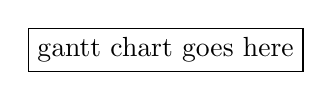
\begin{tikzpicture}
      \node[draw] {gantt chart goes here};
    \end{tikzpicture}
  \caption{Project Gantt Chart}
  \label{fig:gantt}
\end{figure}

Despite best efforts to accurately estimate the amount of time that would be necessary to complete certain tasks, due to lack of experience, some of these were underestimated which meant that, due to time limitations, it was necessary to remove some features from the project scope to ensure that those features which are implemented are completed to a high quality. The Gantt chart served well identifying when tasks were overrunning and could potentially impact the timely delivery of the project as a whole. As the project began falling behind schedule, with tasks such as prototyping the message sending and receiving process taking considerably longer than expected due to the complexitites of the node-imap library, it was decided that file sharing functionality should be excluded from the project scope. This decision was made so that a more essential feature, end-to-end encryption, could be implemented fully and to a high standard, and this was completed on schedule.

Throughout the course of the project, progress was tracked using an online Kanban board on Trello. The benefit of this board is that it was possible to generate a burnup chart, seen in Figure \ref{fig:burnup}, showing the number of work items (cards) completed over time.

Work over the course of the project was relatively consistent, with some time taken for exam revision from December through January. The COVID-19 situation towards the end of the project presented some disruption and uncertainty, however this was primarily during the report writing stage and therefore did not significantly affect progress in terms of development.

\begin{figure}[h!]
  \centering
  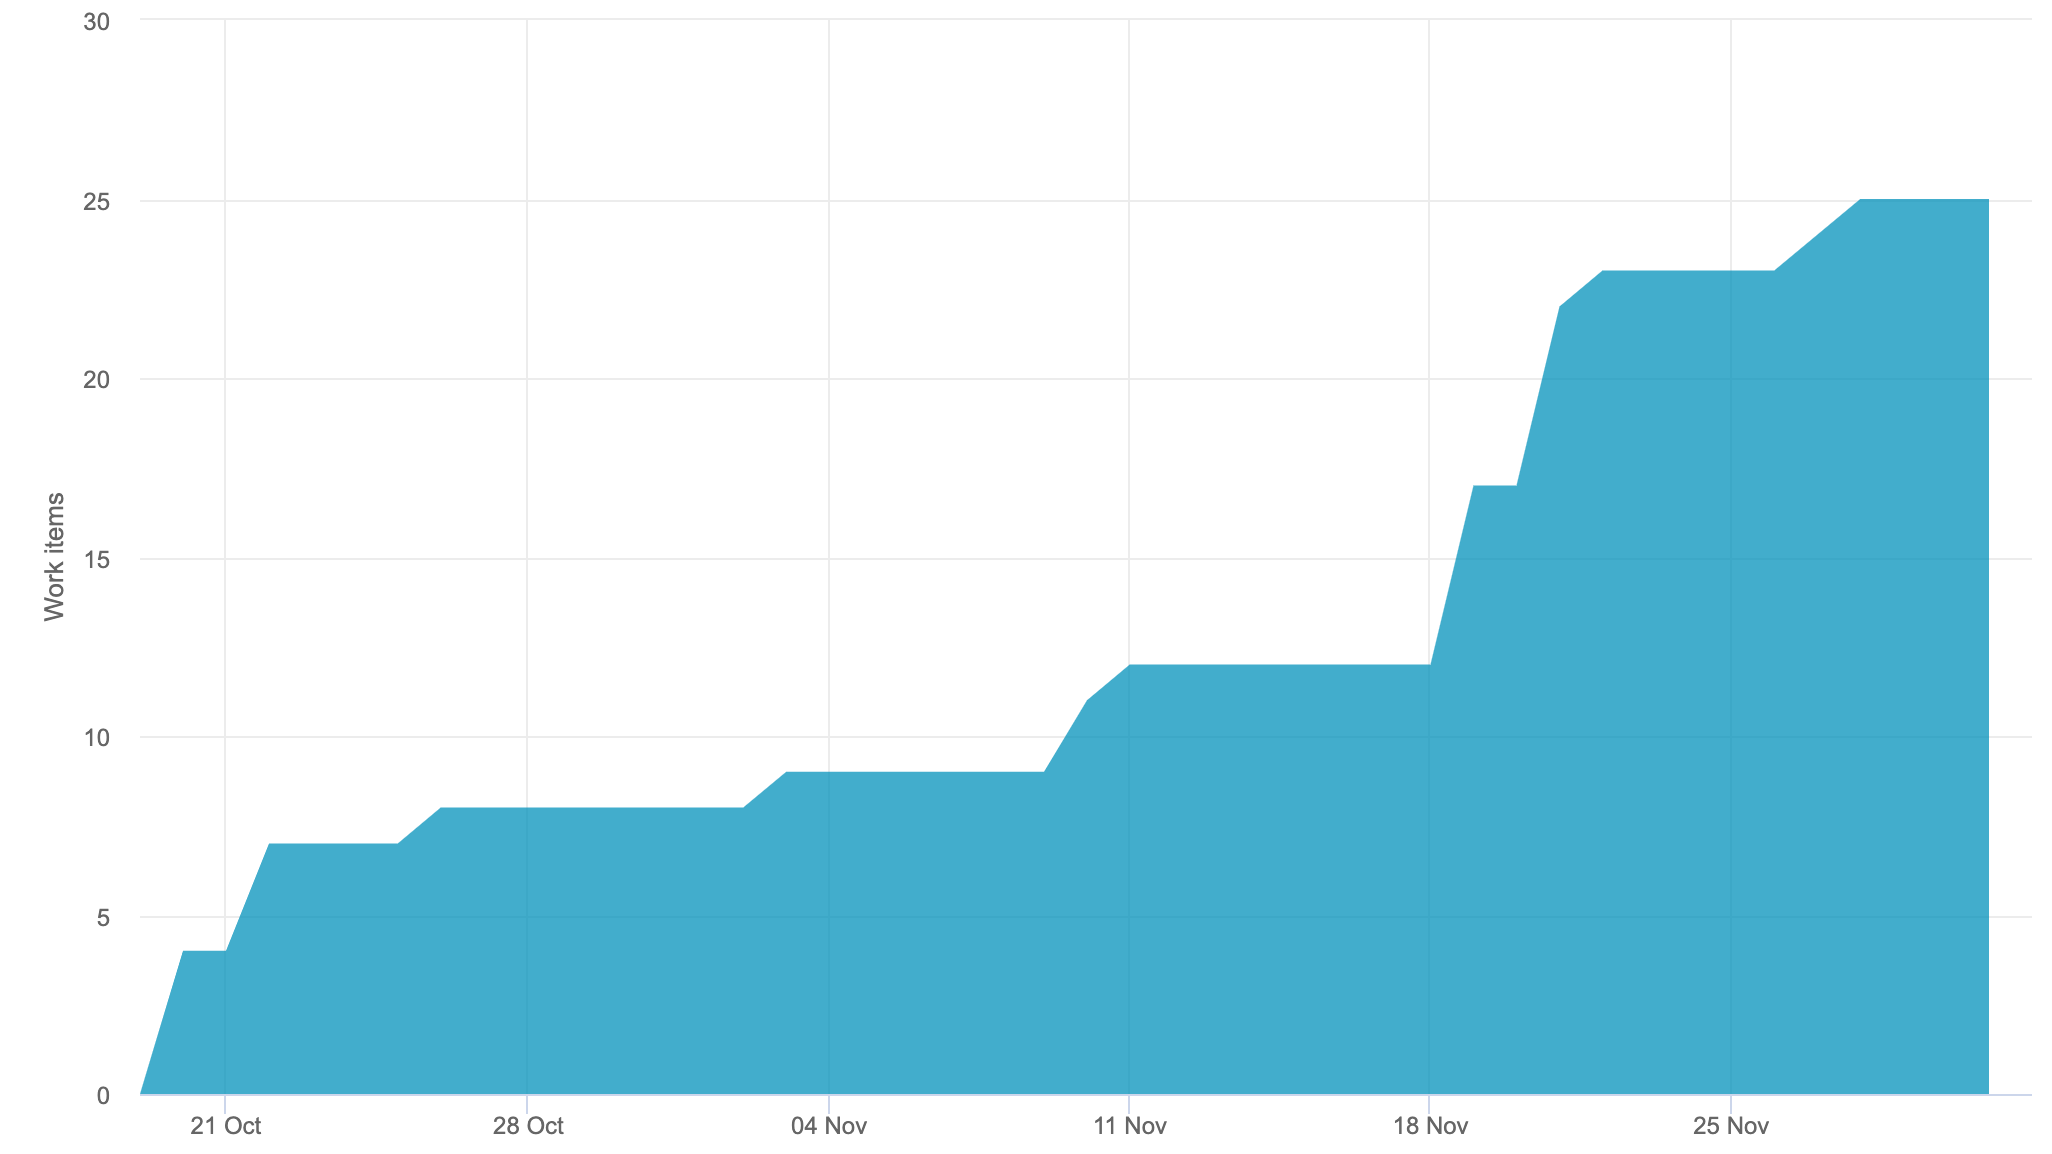
\includegraphics[width=\textwidth]{images/burnup.png}
  \caption{Burnup chart showing number of completed work items over time}
  \label{fig:burnup}
\end{figure}

\section{Contributions and Reflections}

% Providing the details of your achievements and contributions including innovation, creativity and novelty (if there is any) as well as a personal reflection on the plan and your experience of the project (a critical appraisal of how the project went).

Overall, I believe that this project has been a success, with high quality, well tested code, culminating in a software product that meets the vast majority of the initial requirements. Writing unit tests often took a considerable amount of time, and this was not factored into the time estimates for task completion, which did lead to changes to the project plan. The project presented a number of challenges, including developing a user interface that supports an excellent user experience as well as working with complex communication protocols such as IMAP. Designing and implementing effective solutions to these has stretched my abilities as a software engineer and enabled me to explore areas that I had not previously had the opportunity to work in.

\section{Future Work}
Despite the significant work that has taken place so far, there is some further work necessary before this software could become a commercially viable product, and there are additional features that could be added. The immediate focus for future work should be to implement the features that were removed from the project scope for various reasons. Following this, further improvements can be made. In addition, the software would benefit from improvements to the current unit and functional testing coverage, to ensure that all further developments are sufficiently regression tested. Some of the key items of work to be completed in the future are; to allow users to send attachments, as was originally planned, which would help to increase adoption of this platform as a new messaging client. In addition; to improve the application's performance, message fetching should be paginated, so that only a subset of a conversation's messages are fetched to begin with (the most recent), and more messages are fetched as the user scrolls back.
